\documentclass{standalone}

\usepackage{tikz}
\usetikzlibrary{decorations.markings}
\begin{document}



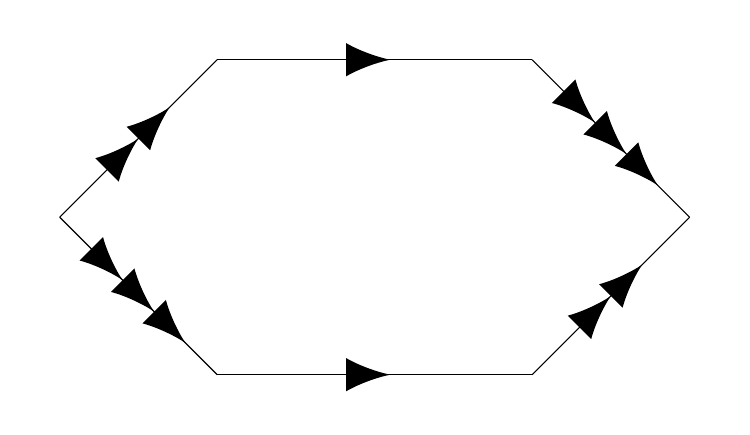
\begin{tikzpicture}[scale=2]

\draw[white] (-1.2,-.2)--(-1.2,-.2);
\draw[white] (3.2,2.2)--(3.2,2.2);

\draw[  
        decoration={markings, mark=at position 0.55 with {\arrow[scale=4]{latex}}},     postaction={decorate}
        ] (0,0)--(2,0);
\draw[        decoration={markings, mark=at position 0.55 with {\arrow[scale=4]{latex}}},     postaction={decorate}] (0,2)--(2,2);
\draw[   decoration={markings, mark=at position 0.5 with {\arrow[scale=4]{latex}}, mark=at position 0.7 with {\arrow[scale=4]{latex}}},    postaction={decorate}] (-1,1)--(0,2);
\draw[   decoration={markings, mark=at position 0.5 with {\arrow[scale=4]{latex}}, mark=at position 0.7 with {\arrow[scale=4]{latex}}},     postaction={decorate}] (2,0)--(3,1);

\draw[ decoration={markings, mark=at position 0.4 with {\arrow[scale=4]{latex}}, mark=at position 0.6 with {\arrow[scale=4]{latex}}, mark=at position 0.8 with {\arrow[scale=4]{latex}}},     postaction={decorate}] (-1,1)--(0,0);

\draw[decoration={markings, mark=at position 0.4 with {\arrow[scale=4]{latex}}, mark=at position 0.6 with {\arrow[scale=4]{latex}}, mark=at position 0.8 with {\arrow[scale=4]{latex}}},     postaction={decorate}] (2,2)--(3,1);




\end{tikzpicture} 


\end{document}
